        %%******************************************%%
        %%                                          %%
        %%        Modello di tesi di laurea         %%
        %%            di Andrea Giraldin            %%
        %%                                          %%
        %%             2 novembre 2012              %%
        %%                                          %%
        %%******************************************%%


% I seguenti commenti speciali impostano:
% 1. 
% 2. PDFLaTeX come motore di composizione;
% 3. tesi.tex come documento principale;
% 4. il controllo ortografico italiano per l'editor.

% !TEX encoding = UTF-8
% !TEX TS-program = pdflatex
% !TEX root = tesi.tex
% !TEX spellcheck = it-IT

\documentclass[10pt,                    % corpo del font principale
               a4paper,                 % carta A4
               twoside,                 % impagina per fronte-retro
               openright,               % inizio capitoli a destra
               english,                 
               italian,                 
               ]{book}    

%**************************************************************
% Importazione package
%************************************************************** 

%\usepackage{amsmath,amssymb,amsthm}    % matematica

\usepackage[T1]{fontenc}                % codifica dei font:
                                        % NOTA BENE! richiede una distribuzione *completa* di LaTeX

\usepackage[utf8]{inputenc}             % codifica di input; anche [latin1] va bene
                                        % NOTA BENE! va accordata con le preferenze dell'editor

\usepackage[english, italian]{babel}    % per scrivere in italiano e in inglese;
                                        % l'ultima lingua (l'italiano) risulta predefinita

\usepackage{bookmark}                   % segnalibri

\usepackage{caption}                    % didascalie

\usepackage{chngpage,calc}              % centra il frontespizio

\usepackage{csquotes}                   % gestisce automaticamente i caratteri (")

\usepackage{emptypage}                  % pagine vuote senza testatina e piede di pagina

\usepackage{epigraph}			% per epigrafi

\usepackage{eurosym}                    % simbolo dell'euro

%\usepackage{indentfirst}               % rientra il primo paragrafo di ogni sezione

\usepackage{graphicx}                   % immagini

\usepackage{hyperref}                   % collegamenti ipertestuali

\usepackage[binding=5mm]{layaureo}      % margini ottimizzati per l'A4; rilegatura di 5 mm

\usepackage{listings}                   % codici

\usepackage{microtype}                  % microtipografia

\usepackage{mparhack,fixltx2e,relsize}  % finezze tipografiche

\usepackage{nameref}                    % visualizza nome dei riferimenti                                      

\usepackage[font=small]{quoting}        % citazioni

\usepackage{subfig}                     % sottofigure, sottotabelle

\usepackage[italian]{varioref}          % riferimenti completi della pagina

\usepackage[dvipsnames]{xcolor}         % colori

\usepackage{booktabs}                   % tabelle                                       
\usepackage{tabularx}                   % tabelle di larghezza prefissata                                    
\usepackage{longtable}                  % tabelle su più pagine                                        
\usepackage{ltxtable}                   % tabelle su più pagine e adattabili in larghezza

\usepackage[toc, acronym]{glossaries}   % glossario
                                        % per includerlo nel documento bisogna:
                                        % 1. compilare una prima volta tesi.tex;
                                        % 2. eseguire: makeindex -s tesi.ist -t tesi.glg -o tesi.gls tesi.glo
                                        % 3. eseguire: makeindex -s tesi.ist -t tesi.alg -o tesi.acr tesi.acn
                                        % 4. compilare due volte tesi.tex.

\usepackage[backend=biber,style=verbose-ibid,hyperref,backref]{biblatex}
                                        % eccellente pacchetto per la bibliografia; 
                                        % produce uno stile di citazione autore-anno; 
                                        % lo stile "numeric-comp" produce riferimenti numerici
                                        % per includerlo nel documento bisogna:
                                        % 1. compilare una prima volta tesi.tex;
                                        % 2. eseguire: biber tesi
                                        % 3. compilare ancora tesi.tex.

%**************************************************************
% file contenente le impostazioni della tesi
%**************************************************************

%**************************************************************
% Frontespizio
%**************************************************************

% Autore
\newcommand{\myName}{Fontolan Carlo}                                    
\newcommand{\myTitle}{Realizzazione di una applicazione di process mining per il filtraggio degli eventi}

% Tipo di tesi                   
\newcommand{\myDegree}{Tesi di laurea triennale}

% Università             
\newcommand{\myUni}{Università degli Studi di Padova}

% Facoltà       
\newcommand{\myFaculty}{Corso di Laurea in Informatica}

% Dipartimento
\newcommand{\myDepartment}{Dipartimento di Matematica "Tullio Levi-Civita"}

% Titolo del relatore
\newcommand{\profTitle}{Prof.}

% Relatore
\newcommand{\myProf}{Tullio Vardanega}

% Luogo
\newcommand{\myLocation}{Padova}

% Anno accademico
\newcommand{\myAA}{2018-2019}

% Data discussione
\newcommand{\myTime}{Dicembre 2019}


%**************************************************************
% Impostazioni di impaginazione
% see: http://wwwcdf.pd.infn.it/AppuntiLinux/a2547.htm
%**************************************************************

\setlength{\parindent}{14pt}   % larghezza rientro della prima riga
\setlength{\parskip}{0pt}   % distanza tra i paragrafi


%**************************************************************
% Impostazioni di biblatex
%**************************************************************
\bibliography{bibliografia} % database di biblatex 

\defbibheading{bibliography} {
    \cleardoublepage
    \phantomsection 
    \addcontentsline{toc}{chapter}{\bibname}
    \chapter*{\bibname\markboth{\bibname}{\bibname}}
}

\setlength\bibitemsep{1.5\itemsep} % spazio tra entry

\DeclareBibliographyCategory{opere}
\DeclareBibliographyCategory{web}

\addtocategory{opere}{womak:lean-thinking}
\addtocategory{web}{site:agile-manifesto}

\defbibheading{opere}{\section*{Riferimenti bibliografici}}
\defbibheading{web}{\section*{Siti Web consultati}}


%**************************************************************
% Impostazioni di caption
%**************************************************************
\captionsetup{
    tableposition=top,
    figureposition=bottom,
    font=small,
    format=hang,
    labelfont=bf
}

%**************************************************************
% Impostazioni di glossaries
%**************************************************************

%**************************************************************
% Glossario
%**************************************************************
%\renewcommand{\glossaryname}{Glossario}

\newglossaryentry{apig}
{
    name=\glslink{api}{API},
    text=Application Program Interface,
    sort=api,
    description={in informatica con il termine \emph{Application Programming Interface API} (ing. interfaccia di programmazione di un'applicazione) si indica ogni insieme di procedure disponibili al programmatore, di solito raggruppate a formare un set di strumenti specifici per l'espletamento di un determinato compito all'interno di un certo programma. La finalità è ottenere un'astrazione, di solito tra l'hardware e il programmatore o tra software a basso e quello ad alto livello semplificando così il lavoro di programmazione}
}



\newglossaryentry{helpdesk}
{
    name=\glslink{helpdesk}{Helpdesk},
    text=helpdesk,
    sort=helpdesk,
    description={Servizio clienti telematico}
}

\newglossaryentry{tfs}
{
    name=\glslink{tfs}{TFS},
    text=TFS,
    sort=Tfs,
    description={Team foundation server}
}

\newglossaryentry{tfvc}
{
    name=\glslink{tfvc}{TFVC},
    text=TFVC,
    sort=Tfvc,
    description={Team foundation version control}
}
\newglossaryentry{deploy}
{
    name=\glslink{deploy}{Deploy},
    text=deploy,
    sort=deploy,
    description={ consegna o rilascio al cliente, con relativa installazione e messa in funzione o esercizio, di una applicazione o di un sistema software tipicamente all'interno di un sistema informatico aziendale}
}

\newglossaryentry{Angular}
{
    name=\glslink{Angular}{Angular},
    text=Angular,
    sort=Angular,
    description={ Angular 2+ è una piattaforma open source per lo sviluppo di applicazioni web con licenza MIT, evoluzione di AngularJS. Sviluppato principalmente da Google, la sua prima release è avvenuta il 14 settembre 2016}
}

\newglossaryentry{Websocket}
{
    name=\glslink{Websocket}{Websocket},
    text=Websocket,
    sort=Websocket,
    description={tecnologia web che fornisce canali di comunicazione full-duplex attraverso una singola connessione TCP}
}
\newglossaryentry{Cloud}
{
    name=\glslink{Cloud}{Cloud},
    text=Cloud,
    sort=Cloud,
    description={paradigma di erogazione di servizi offerti on demand da un fornitore ad un cliente finale attraverso la rete Internet}
}

\newglossaryentry{BigData}
{
    name=\glslink{BigData}{BigData},
    text=BigData,
    sort=BigData,
    description={raccolta estesa di dati in termini di volume, velocità e varietà da richiedere tecnologie e metodi analitici specifici per l'estrazione di valore o conoscenza}
}

\newglossaryentry{Framework}
{
    name=\glslink{Framework}{Framework},
    text=Framework,
    sort=Framework,
    description={Architettura logica di supporto su cui un software può essere progettato e realizzato}
}

\newglossaryentry{Broker}
{
    name=\glslink{Broker}{Broker},
    text=Broker,
    sort=Broker,
    description={Sistema che distribuisce vari aspetti del software su nodi differenti tramite l'utilizzo di oggetti remoti}
}

\newglossaryentry{Stage-IT}
{
    name=\glslink{Stage-IT}{Stage-IT},
    text=Stage-IT,
    sort=Stage-IT,
    description={Evento organizzate presso Padova Fiere in collaborazione con varie aziende locali che cercano di far approcciare gli studenti al mondo lavorativo tramite attività di stage}
}
\newglossaryentry{Javadoc}
{
    name=\glslink{Javadoc}{Javadoc},
    text=Javadoc,
    sort=Javadoc,
    description={Javadoc è un applicativo incluso all'interno del Java Development Kit della Sun Microsystems, utilizzato per la generazione automatica della documentazione del codice sorgente scritto in linguaggio Java}
}
\newglossaryentry{stub}
{
    name=\glslink{stub}{Stub},
    text=stub,
    sort=stub,
    description={è una porzione di codice utilizzata in sostituzione di altre funzionalità software in quanto può simulare il comportamento di codice esistente o l'interfaccia COM, e temporaneo sostituto di codice ancora da sviluppare}
}
\newglossaryentry{callback}
{
    name=\glslink{callback}{Callback},
    text=callback,
    sort=callback,
    description={funzione o blocco di codice che viene passato come parametro ad un'altra funzione}
}
\newglossaryentry{Disco}
{
    name=\glslink{Disco}{Disco},
    text=Disco,
    sort=Disco,
    description={Tool di process mining sviluppato da Fluxicon}
}

\newglossaryentry{JSON}
{
    name=\glslink{JSON}{JSON},
    text=JSON,
    sort=JSON,
    description={JavaScript Object Notation. Formato adatto all'interscambio di applicazione client/server}
}

\newglossaryentry{unit test}
{
    name=\glslink{unit test}{Unit test},
    text=unit test,
    sort=unit test,
    description={l'attività di testing di singole unità software.}
}
\newglossaryentry{mockup}
{
    name=\glslink{mockup}{Mockup},
    text=mockup,
    sort=mockup,
    description={realizzazione a scopo illustrativo di un oggetto o sistema senza le complete funzioni originali}
}
\newglossaryentry{open-closed}
{
    name=\glslink{open-closed}{Open-closed},
    text=open-closed,
    sort=open-closed,
    description={principio cardine di S.O.L.I.D \textit{principle} attraverso il quale un sistema deve essere aperto alle estensioni ma chiuso alle modifiche.}
} % database di termini
\makeglossaries


%**************************************************************
% Impostazioni di graphicx
%**************************************************************
\graphicspath{{immagini/}} % cartella dove sono riposte le immagini


%**************************************************************
% Impostazioni di hyperref
%**************************************************************
\hypersetup{
    %hyperfootnotes=false,
    %pdfpagelabels,
    %draft,	% = elimina tutti i link (utile per stampe in bianco e nero)
    colorlinks=true,
    linktocpage=true,
    pdfstartpage=1,
    pdfstartview=FitV,
    % decommenta la riga seguente per avere link in nero (per esempio per la stampa in bianco e nero)
    %colorlinks=false, linktocpage=false, pdfborder={0 0 0}, pdfstartpage=1, pdfstartview=FitV,
    breaklinks=true,
    pdfpagemode=UseNone,
    pageanchor=true,
    pdfpagemode=UseOutlines,
    plainpages=false,
    bookmarksnumbered,
    bookmarksopen=true,
    bookmarksopenlevel=1,
    hypertexnames=true,
    pdfhighlight=/O,
    %nesting=true,
    %frenchlinks,
    urlcolor=webbrown,
    linkcolor=RoyalBlue,
    citecolor=webgreen,
    %pagecolor=RoyalBlue,
    %urlcolor=Black, linkcolor=Black, citecolor=Black, %pagecolor=Black,
    pdftitle={\myTitle},
    pdfauthor={\textcopyright\ \myName, \myUni, \myFaculty},
    pdfsubject={},
    pdfkeywords={},
    pdfcreator={pdfLaTeX},
    pdfproducer={LaTeX}
}

%**************************************************************
% Impostazioni di itemize
%**************************************************************
\renewcommand{\labelitemi}{$\ast$}

%\renewcommand{\labelitemi}{$\bullet$}
%\renewcommand{\labelitemii}{$\cdot$}
%\renewcommand{\labelitemiii}{$\diamond$}
%\renewcommand{\labelitemiv}{$\ast$}


%**************************************************************
% Impostazioni di listings
%**************************************************************
\lstset{
    language=[LaTeX]Tex,%C++,
    keywordstyle=\color{RoyalBlue}, %\bfseries,
    basicstyle=\small\ttfamily,
    %identifierstyle=\color{NavyBlue},
    commentstyle=\color{Green}\ttfamily,
    stringstyle=\rmfamily,
    numbers=none, %left,%
    numberstyle=\scriptsize, %\tiny
    stepnumber=5,
    numbersep=8pt,
    showstringspaces=false,
    breaklines=true,
    frameround=ftff,
    frame=single
} 


%**************************************************************
% Impostazioni di xcolor
%**************************************************************
\definecolor{webgreen}{rgb}{0,.5,0}
\definecolor{webbrown}{rgb}{.6,0,0}


%**************************************************************
% Altro
%**************************************************************

\newcommand{\omissis}{[\dots\negthinspace]} % produce [...]

% eccezioni all'algoritmo di sillabazione
\hyphenation
{
    ma-cro-istru-zio-ne
    gi-ral-din
}

\newcommand{\sectionname}{sezione}
\addto\captionsitalian{\renewcommand{\figurename}{Figura}
                       \renewcommand{\tablename}{Tabella}}

\newcommand{\glsfirstoccur}{\ap{{[g]}}}

\newcommand{\intro}[1]{\emph{\textsf{#1}}}

%**************************************************************
% Environment per ``rischi''
%**************************************************************
\newcounter{riskcounter}                % define a counter
\setcounter{riskcounter}{0}             % set the counter to some initial value

%%%% Parameters
% #1: Title
\newenvironment{risk}[1]{
    \refstepcounter{riskcounter}        % increment counter
    \par \noindent                      % start new paragraph
    \textbf{\arabic{riskcounter}. #1}   % display the title before the 
                                        % content of the environment is displayed 
}{
    \par\medskip
}

\newcommand{\riskname}{Rischio}

\newcommand{\riskdescription}[1]{\textbf{\\Descrizione:} #1.}

\newcommand{\risksolution}[1]{\textbf{\\Soluzione:} #1.}

%**************************************************************
% Environment per ``use case''
%**************************************************************
\newcounter{usecasecounter}             % define a counter
\setcounter{usecasecounter}{0}          % set the counter to some initial value

%%%% Parameters
% #1: ID
% #2: Nome
\newenvironment{usecase}[2]{
    \renewcommand{\theusecasecounter}{\usecasename #1}  % this is where the display of 
                                                        % the counter is overwritten/modified
    \refstepcounter{usecasecounter}             % increment counter
    \vspace{10pt}
    \par \noindent                              % start new paragraph
    {\large \textbf{\usecasename #1: #2}}       % display the title before the 
                                                % content of the environment is displayed 
    \medskip
}{
    \medskip
}

\newcommand{\usecasename}{UC}

\newcommand{\usecaseactors}[1]{\textbf{\\Attori Principali:} #1. \vspace{4pt}}
\newcommand{\usecasepre}[1]{\textbf{\\Precondizioni:} #1. \vspace{4pt}}
\newcommand{\usecasedesc}[1]{\textbf{\\Descrizione:} #1. \vspace{4pt}}
\newcommand{\usecasepost}[1]{\textbf{\\Postcondizioni:} #1. \vspace{4pt}}
\newcommand{\usecasealt}[1]{\textbf{\\Scenario Alternativo:} #1. \vspace{4pt}}

%**************************************************************
% Environment per ``namespace description''
%**************************************************************

\newenvironment{namespacedesc}{
    \vspace{10pt}
    \par \noindent                              % start new paragraph
    \begin{description} 
}{
    \end{description}
    \medskip
}

\newcommand{\classdesc}[2]{\item[\textbf{#1:}] #2}                     % file con le impostazioni personali

\begin{document}
%**************************************************************
% Materiale iniziale
%**************************************************************
\frontmatter
% !TEX encoding = UTF-8
% !TEX TS-program = pdflatex
% !TEX root = ../tesi.tex

%**************************************************************
% Frontespizio 
%**************************************************************
\begin{titlepage}

\begin{center}

\begin{LARGE}
\textbf{\myUni}\\
\end{LARGE}

\vspace{10pt}

\begin{Large}
\textsc{\myDepartment}\\
\end{Large}

\vspace{10pt}

\begin{large}
\textsc{\myFaculty}\\
\end{large}

\vspace{30pt}
\begin{figure}[htbp]
\begin{center}

\includegraphics[height=6cm]{logo-unipd}
\end{center}
\end{figure}
\vspace{30pt} 

\begin{LARGE}
\begin{center}
\textbf{\myTitle}\\
\end{center}
\end{LARGE}

\vspace{10pt} 

\begin{large}
\textsl{\myDegree}\\
\end{large}

\vspace{40pt} 

\begin{large}
\begin{flushleft}
\textit{Relatore}\\ 
\vspace{5pt} 
\profTitle \myProf
\end{flushleft}

\vspace{0pt} 

\begin{flushright}
\textit{Laureando}\\ 
\vspace{5pt} 
\myName
\end{flushright}
\end{large}

\vspace{21pt}

\line(1, 0){338} \\
\begin{normalsize}
\textsc{Anno Accademico \myAA}
\end{normalsize}

\end{center}
\end{titlepage} 
% !TEX encoding = UTF-8
% !TEX TS-program = pdflatex
% !TEX root = ../tesi.tex

%**************************************************************
% Colophon
%**************************************************************
\clearpage
\phantomsection
\thispagestyle{empty}

\hfill

\vfill

\noindent\myName: \textit{\myTitle,}
\myDegree,
\textcopyright\ \myTime.
%% !TEX encoding = UTF-8
% !TEX TS-program = pdflatex
% !TEX root = ../tesi.tex

%**************************************************************
% Dedica
%**************************************************************
\cleardoublepage
\phantomsection
\thispagestyle{empty}
\pdfbookmark{Dedica}{Dedica}

\vspace*{3cm}

\begin{center}
Lorem ipsum dolor sit amet, consectetuer adipiscing elit. \\ \medskip
--- Oscar Wilde    
\end{center}

\medskip

\begin{center}
Dedicato a ...
\end{center}

% !TEX encoding = UTF-8
% !TEX TS-program = pdflatex
% !TEX root = ../tesi.tex

%**************************************************************
% Sommario
%**************************************************************
\cleardoublepage
\phantomsection
\pdfbookmark{Sommario}{Sommario}
\begingroup
\let\clearpage\relax
\let\cleardoublepage\relax
\let\cleardoublepage\relax

\chapter*{Sommario}

Il presente documento descrive il lavoro svolto durante il periodo di stage, della durata di circa trecento ore, dal laureando Pinco Pallino presso l'azienda Azienda S.p.A.
Gli obbiettivi da raggiungere erano molteplici.\\
In primo luogo era richiesto lo sviluppo di ...
In secondo luogo era richiesta l'implementazione di un ... 
Tale framework permette di registrare gli eventi di un controllore programmabile, quali segnali applicati 
Terzo ed ultimo obbiettivo era l'integrazione ...

%\vfill
%
%\selectlanguage{english}
%\pdfbookmark{Abstract}{Abstract}
%\chapter*{Abstract}
%
%\selectlanguage{italian}

\endgroup			

\vfill


% !TEX encoding = UTF-8
% !TEX TS-program = pdflatex
% !TEX root = ../tesi.tex

%**************************************************************
% Ringraziamenti
%**************************************************************
\cleardoublepage
\phantomsection
\pdfbookmark{Ringraziamenti}{ringraziamenti}

%\begin{flushright}{
%	``Life is really simple, but we insist on making it complicated''} \\ 
%	\medskip
%    --- Confucius
%\end{flushright}


\bigskip

\begingroup
\let\clearpage\relax
\let\cleardoublepage\relax
\let\cleardoublepage\relax

\chapter*{Ringraziamenti}

\noindent \textit{Innanzitutto, vorrei esprimere la mia gratitudine al Prof. \myProf, relatore della mia tesi, per l'aiuto e il sostegno fornitomi durante la stesura del lavoro.}\\

\noindent \textit{Desidero ringraziare con affetto i miei genitori per il sostegno, il grande aiuto e per essermi stati vicini in ogni momento durante gli anni di studio.}\\

\noindent \textit{Ho desiderio di ringraziare poi i miei amici per tutti i bellissimi anni passati insieme e le mille avventure vissute.}\\
\bigskip

\noindent\textit{\myLocation, \myTime}
\hfill \myName

\endgroup


% !TEX encoding = UTF-8
% !TEX TS-program = pdflatex
% !TEX root = ../tesi.tex

%**************************************************************
% Indici
%**************************************************************
\cleardoublepage
\pdfbookmark{\contentsname}{tableofcontents}
\setcounter{tocdepth}{2}
\tableofcontents
%\markboth{\contentsname}{\contentsname} 
\clearpage

\begingroup 
    \let\clearpage\relax
    \let\cleardoublepage\relax
    \let\cleardoublepage\relax
    %*******************************************************
    % Elenco delle figure
    %*******************************************************    
    \phantomsection
    \pdfbookmark{\listfigurename}{lof}
    \listoffigures

    \vspace*{8ex}

    %*******************************************************
    % Elenco delle tabelle
    %*******************************************************
    \phantomsection
    \pdfbookmark{\listtablename}{lot}
    \listoftables
        
    \vspace*{8ex}
\endgroup

\cleardoublepage

\cleardoublepage

%**************************************************************
% Materiale principale
%**************************************************************
\mainmatter
% !TEX encoding = UTF-8
% !TEX TS-program = pdflatex
% !TEX root = ../tesi.tex

%**************************************************************
\chapter{Il contesto aziendale}
\section{L'azienda}
Siav è una delle più importanti realtà italiane di sviluppo software e di servizi informatici
specializzata nella dematerializzazione e nella gestione documentale e nei processi
digitali. Presenta diverse filiali nel suolo italiano che cooperano tra loro per un fine comune. Siav inoltre punta molto sulla collaborazione tra aziende, in campo nazionale sia a livello pubblico che privato, ma anche a livello internazionale. Una fra tutti Microsoft.
I loro servizi puntano in primo luogo, ad una miglior gestione, controllo ed automazione di tutti i principali processi aziendali; in secondo luogo, ad offrire diverse soluzioni concrete anche a singoli privati che necessitano di sistemi di gestione ed integrazione per lo loro piccola realtà.
\begin{figure}[!h] 
	\centering 
	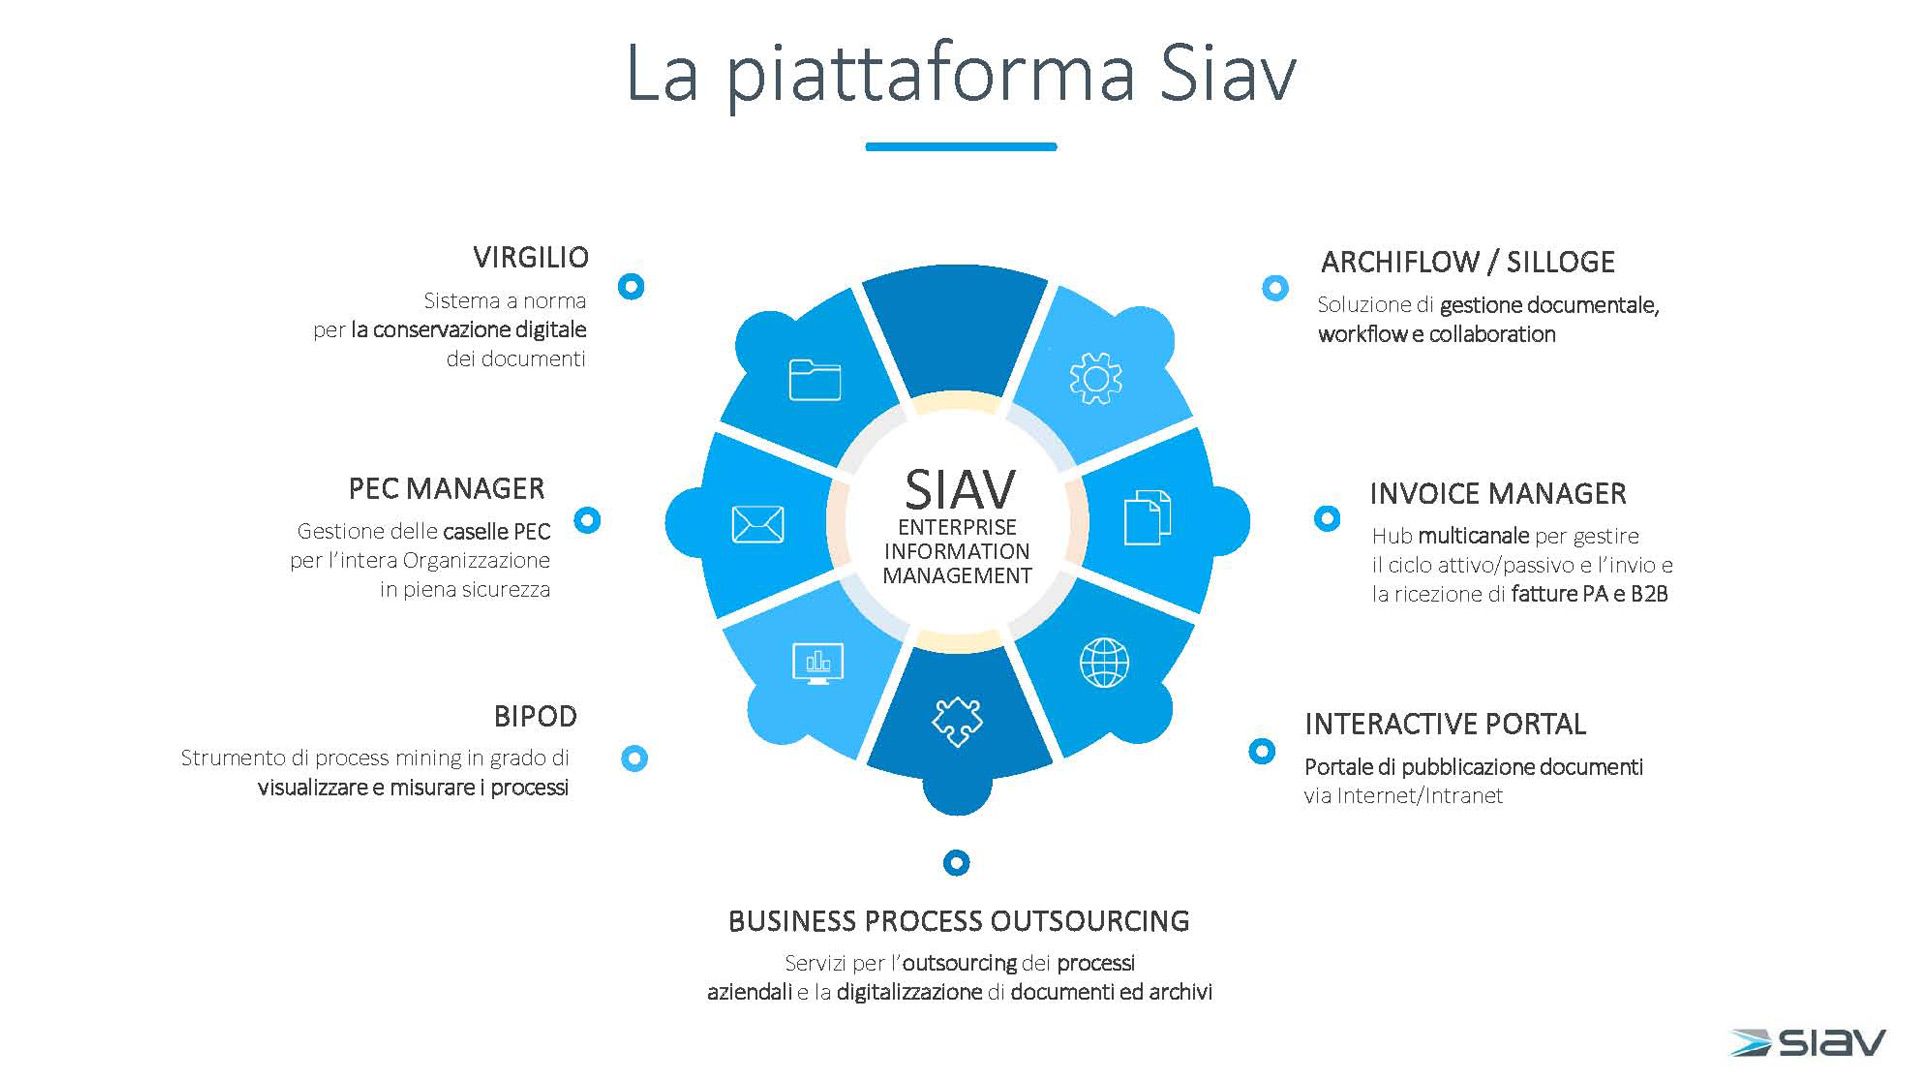
\includegraphics[width=1.15\columnwidth]{siav} 
	\caption{I prodotti offerti da Siav (\url{https://tinyurl.com/sm45xtu})}
\end{figure}
Siav si colloca all'interno del mercato come una tra la più importanti realtà italiane a livello di \textit{Enterprise Content Management} offrendo servizi per poter migliorare processi e gestioni aziendali spaziando da un gestore di caselle PEC, ad un applicativo di process mining denominato \textit{Bipod}, fino ad arrivare al loro prodotto di punta: Archiflow/Silloge: un software in continuo sviluppo, mantenuto e aggiornato da piccoli team che lavorano in sinergia per raggiungere un obiettivo comune. Archiflow/Silloge offre una soluzione alla gestione di una cospicua mole di documenti, categorizzandoli in varie sezioni permettendone un facile reperimento.
\section{Clientela rivolta a Siav}
La maggior parte dei clienti che si affidano a \textit{Siav} sono aziende che presentano il bisogno di automatizzarsi e migliorare i propri processi interni andando cosi ad incrementare la propria efficenza sotto l'aspetto lavorativo. Tali aziende sono di vario genere con diverse necessità, dal semplice ristorante ad una nota catena di supermercati fino ad aziende metalmeccaniche. Per ogni settore, l'azienda è in continua ricerca di nuove opportunità e soluzioni che possano potare a miglioramenti aziendali, cercando di spaziare verso più ambienti lavorativi, allargando sempre più il proprio campo applicativo per portare verso di sè una clientela più varia. Questo ha portato l'azienda a dover standardizzare i propri prodotti in modo da poter coinvolgere una maggior porzione di clientela, per ogni settore.
Siav è catalogata come \textit{Software house} e presenta un ampio catalogo di prodotti atti a soddisfare le principali necessità organizzative e gestionali di un'azienda, sta al potenziale cliente poi, valutarne l'acquisto in base alle proprie necessità.
\newpage
\section {Processi aziendali}
In questa sezione sono descritti i pricipali processi e strumenti che ho visto utilizzare all'interno dell'azieda durante il mio periodo di permanenza, dividendoli in metodologie e strumenti.
\subsection{Metodologie di sviluppo}
L'azienda normalmente si ritrova a dover far fronte ad alcune problematiche derivate da bug, criticità o variazioni importanti di requisiti che possono essere riscontrate durante i vari processi aziendali ed incidere in modo significativo sull'andamento dello sviluppo.
Per cercare di venire incontro a ciò l'azienda ha adottato una metodologia di tipo \textit{Agile}, cercando di mantenere un atteggiamento flessibile rispetto ai processi e gli obiettivi. Risulta quindi fondamentale l'organizzazione di incontri durante vari momenti della giornata o settimana in modo da confrontarsi sull'andamento dei processi e lo stato di avanzamento del prodotto. È consuetudine dei team di lavoro un confronto giornaliero tramite \textit{daily meeting}, per discutere su quanto fatto durante la giornata precedente indicando le eventuali criticità riscontrate, pianificando cosi gli obiettivi per la giornata odierna. Ad inizio settimana invece viene organizzato un \textit{weekly meeting} per constatare gli stati di avanzamento rispetto alla settimana precedente, per poi fissare gli obiettivi per la settimana successiva. Gli obiettivi, le attività preposte e le scadenza prefissate a livello complessivo di team vengono solitamente appesi in una lavagna posta in luogo ben visibile all'interno del reparto di sviluppo, per ordine di priorità; in questo modo è quindi possibile tener sott'occhio le principali attività. Il rapporto con il cliente è di vitale importanza per \textit{Siav}. L'azienda infatti presente un servizio di assistenza clienti tramite il quale vengono effettuate segnalazioni di \textit{bug} o assistenza sui proprio prodotti 
\begin{figure}[!h] 
	\centering 
	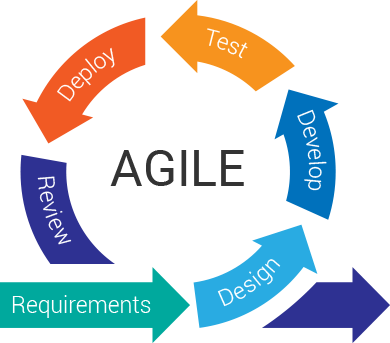
\includegraphics[width=0.4\columnwidth]{agile} 
	\caption{Ciclo di vita della metodologia Agile (\url{https://tinyurl.com/tkqyaww})}
\end{figure}
\subsection{Strumenti di supporto }
L'azienda mette a disposizione diversi strumenti di supporto, allo scopo di gestire e tenere traccia nel migliore dei modi tutte le attività di progetto.
Facendo fede alla metodologia \textit{Agile}, la maggior parte degli strumenti servono a gestire tutti gli aspetti che riguardano il codice. Viene utilizzato \gls{tfs}, uno strumento di \textit{Microsoft} per la gestione delle principali attivtà di progetto che offre un set di strumenti per la collaborazione. Tra le principali funzionalità offerte sono presenti: gestione del repository tramite tecnologie Git o \gls{tfvc}, gestione dei requisiti e strumenti di \textit{build} automatizzati. Tale strumento aderisce in maniera completa alle tecniche \textit{agile}, andando quindi ad integrarsi in modo solido all'interno della realtà lavorativa. Per quanto riguarda il tracciamente delle attività viene utilizzato \textit{Evernote}: un software che permette la scrittura e la condivisione di note all'interno di un gruppo di utenti. Cosi facendo ogni membro del team di sviluppo ha sotto controllo ogni attività svolta dagli altri membri. Un ulteriore strumento utilizzato per il tracciamento dello attività è \textit{Google Docs}. Tramite quest'ultimo è possibile assegnare attività a tutti i membri che possiedono i privilegi per accedere al documento in questione. Solitamente i task assegnati presentano una struttura semplice: la data di creazione, la possibilità o meno di menzionare direttamente l'interessato a cui risulta assegnato il task ed un casella di risposta per poter descrivere la sua effettiva terminazione, oppure un messaggio di testo di altro genere, che solitamente indica le problematiche per cui il task non è stato possibile risolverlo. \textit{Google Docs} non è l'unico strumento di \textit{ticketing} che utilizza l'azienda ma è stato quello che ho potuto visionare durante il priodo di stage.\\
Per poter garantire una cooperazione efficente tra tutto il personale viene spesso utilizzato \textit{TeamViewer}: un software per il controllo e la gestire altre macchine da remoto, in questo modo è possibile raggiungere un buon grado di cooperazione tra il personale dell'azienda, pur trovandosi in filiali diverse. Tale metodologia viene spesso utilizzata anche all'interno dell'area di \textit{testing} per fornire assistenza immediata ai clienti.

\section {Tecnologie utilizzate}
Le tecnologie utilizzate dell'azienda per la realizzazione dei propri prodotti sono fondate principalmente sulla possibilità di un utilizzo tramite \textit{\gls{Cloud}}, dedicandosi principalmente sullo sviluppo di \textit{Webapp}; dovendo fornire servizi di tipo gestionali e organizzativi l'azienda si trova spesso a dover far fronte alla gestione dei cosiddetti \textit{\gls{BigData}}: fattore crucuiale per \textit{Siav} che interessa la maggior parte dei propri prodotti. Per far fronte a tali problemi l'azienda utilizzia tecnologie innovative e all'avanguardia. Quest'ultime possono essere raggruppate in due macrocategorie: \textit{Front-end} e \textit{Back-end}.
\subsection{\textit{Front-end}}
Da quel che ho potuto constatare durante l'attività di stage, per quanto riguarda lo sviluppo web lato \textit{client} viene utilizzata prevalentamente la piattaforma \textit{\gls{Angular}}.
Quest'ultima è ideale per lo sviluppo di \textit{webapp} multipiattaforma, offrendo diverse funzionalità allo sviluppatore, potendosi adattare a svariate tipologie di architetture.
 Tramite il consistente numero di componenti prefabbricati presenti in rete e una vasta gamma di funzionalità e servizi disponibili, è possibile sviluppare un'interfaccia \textit{front-end} solida e di qualità, soddisfando nel miglior modo possibile le aspettative del cliente. Un'altro aspetto fondmentale di tale \textit{\gls{Framework}} è la possibilità di essere utilizzato su più dispositivi, non restringendo quindi il campo applicativo di \textit{Siav} al solo \textit{Desktop o Laptop} ma spaziando verso tutti principali dispositivi presenti sul mercato.

\subsection{\textit{Back-end}}
Per quanto riguarda lato back-end vengono utilizzate molteplici tecnologie in base alle necessità che prevede il software di sviluppo;  \textit{RabbitMQ}: questa tecnologia è stata pensata principalmente per un'architettura a microservizi e viene utilizzata in più prodotti all'interno dell'azienda. \textit{RabbitMQ} viene definito come un \textit{\gls{Broker}} di messaggisticia: ossia un sistema che monitora la trasmissioni di messaggi tra servizi attraverso una coda in cui vengono memorizzate i messaggi prima di essere inviati.\\ Un'altro sistema utilizzato, restando in ambito di microservizi è \textit{Kubernetes}: un sistema per la gestione di \textit{container} che viene utilizzato dall'azienda per effettuare la duplicazione di contenitori in modo da far fronte ad una cospicua mole di operazioni e richieste da parte di utenti. Per poter sfruttare al massimo l'ambiente \textit{Cloud}, su cui \textit{Siav} investe molte risorse, viene utilizzato \textit{Apache Kafka}: tale sistema è in grando di gestire un gran numero di operazioni in tempo reali provienienti da diversi \textit{Client}, sia per quanto rigaurda la fase di lettura che scrittura. L'azienda quindi cura molto le tecnologie che utilizza all'interno del propri prodotti cercando di trarne il massimo vantaggio da ognuna di esse. 

\begin{figure}[!h] 
	\centering 
	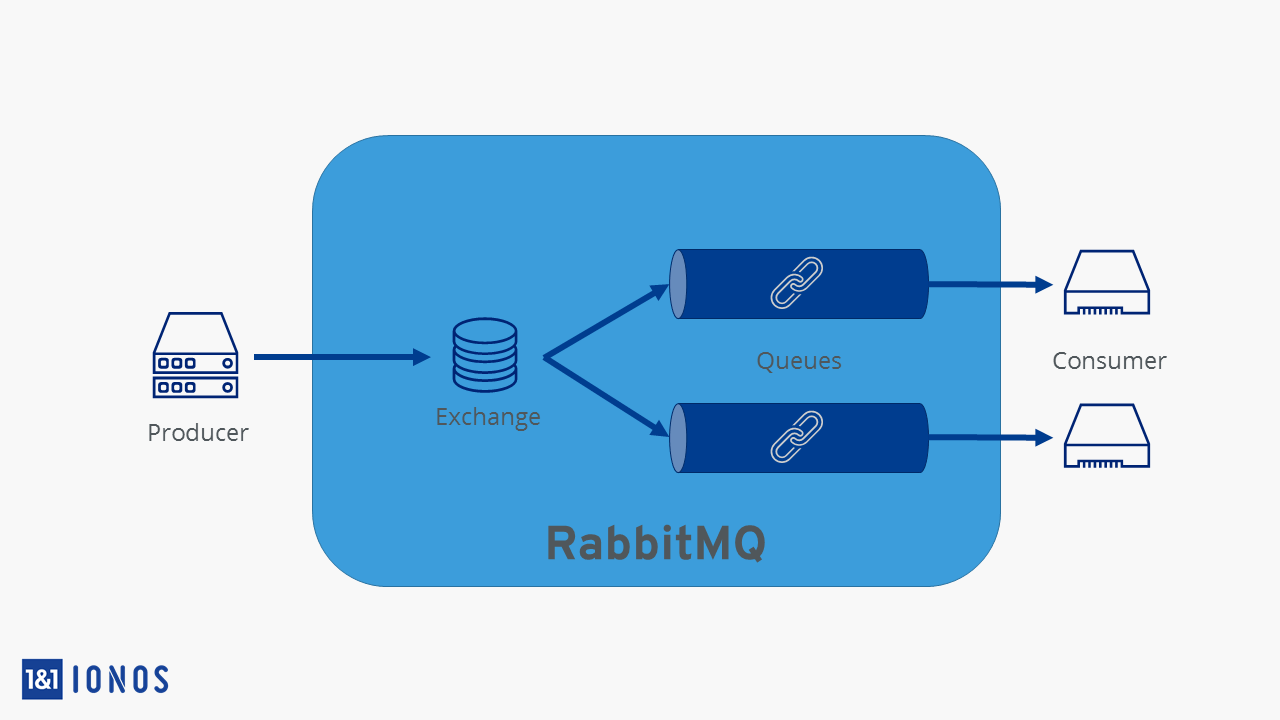
\includegraphics[width=0.9\columnwidth]{rabbitmq} 
	\caption{Diagramm illustrativo sul funzionamento di RabbitMQ
	(\url{https://www.ionos.it/digitalguide/siti-web/programmazione-del-sito-web/rabbitmq/})}
\end{figure}
\section{Propensione all'innovazione}
\textit{Siav} è un'azienda che fa dell'innovazione un suo punto cardine. I prodotti che offre sono costantemente aggiornati, cercando di adattarsi alle necessità del cliente. Per poter far ciò l'azienda ha messo a disposizione un serivizio di \textit{\gls{helpdesk}} in modo da fornire assistenza in merito ai propri prodotti per i propri clienti. L'azienda inoltre è alla continua ricerca di nuove tecnologie per poterle integrare all'interno dei propri applicativi; è presente all'interno dell'organico un team di ricerca e sviluppo che analizza, le varie piattaforme e tecnologie presenti sul mercato. Spesso e volentieri tali attività vengono contestualizzate all'interno di proposte di stage, in modo da poter osservare nel concreto se gli studi e le ricerche fatte in precedenza possano portare a benefici per i prodotti dell'azienda, facendo anche un'attenta analisi dei costi.              % Introduzione
% !TEX encoding = UTF-8
% !TEX TS-program = pdflatex
% !TEX root = ../tesi.tex

%**************************************************************
\chapter{L'attività di stage all'interno della strategia aziendale}
\label{cap:processi-metodologie}
%**************************************************************
\intro{Introduzione al capitolo}\\
  In questo capitolo si andrà ad illustrare la propensione dell'azienda rispetto allo stage, indicando le attività con le relative tematiche che mi sono state proposte e come tali siano inserite all'interno della strategia aziendale\\

%**************************************************************
\section{Vantaggi aziendali}
\textit{Siav} da molti anni ha stretto un accordo con l'Università di Padova per quanto riguarda la propensione a svolgere attività di stage. È in continua ricerca di nuove figure da poter inserire all'interno del loro organigramma, soprattutto per quanto riguarda studenti o neo laureati.  Essendo un'azienda in forte crescita ed espansione, necessita costantemente di nuovo personale, ma soprattutto, di nuove idee e tecnologie da da poter poi mettere in pratica nei loro prodotti. La maggior parte degli stage viene attuata dal settore di Ricerca e Sviluppo proprio per soddisfare questa necessità; solitamente le attività di stage proposte comprendono un periodo di formazione iniziale per poter prendere dimestichezza con le nuove tecnologie che si andranno ad attuare, per poi metterle in pratica con il supporto costante del team. Questa sezione presente all'interno di \textit{Siav} garantisce una costante dedizione alla ricerca, non soffermandosi a ciò che è già presente all'interno dell'azienda, ma cercando di spaziare tra più tematiche in contemporanea, procedendo all'attivazione di più stage in ambiti diversi, spaziando quindi la ricerca su più fronti. L'azienda, inoltre, avendo stipulato un cospicuo numero di \textit{partnership} si ritrova spesso e volentieri a partecipare a diversi \textit{meeting} o seminari per quanto riguarda lo studio e approfondimento di nuove tecnologie emergenti o di tendenza. Tali aspetti vengono poi valutati dal team tramite un studio di fattibilità per poter verificare se le tematiche affrontate possono portare qualcosa di redditizio all'interno del contesto aziendale. Quest'ultime portano \textit{Siav} ad essere una delle realtà italiane più attive e propense alla ricerca e allo sviluppo.

\section{Introduzione al progetto}
\textit{Siav} attraverso i numerosi progetti di stage mira ad esplorare nuove tematiche e nuove opportunità tecnologiche che possano portare ad un miglioramento dei propri prodotti. Il progetto che mi è stato proposto mirava proprio al miglioramento di un loro applicativo. Lo scopo dello stage, è stato diviso in tre parti:
\begin{itemize}
	\item sviluppo di una libreria di \textit{process mining} per la pulizia di log degli eventi
	\item sviluppo di un'interfaccia \textit{frontend} che rispettasse le tematiche presenti all'interno della libreria
	\item sviluppo di stub che simulino il comportamento del \textit{backend} per verificare il corretto funzionamento dell'interfaccia.
\end{itemize}
Tramite questo stage è stato possibile per \textit{Siav} migliorare uno dei propri prodotti che aveva perso la sua mantenibilià, essendo stato sviluppato da un piccolo team che ora non era più presente in azienda. Oltretutto la documentazione è risultata scarsa e di difficile comprensione; è stato quindi deciso di riscrivere l'applicativo da zero, cercando di mantenere le principali funzionalità, analizzando qualche aspetto critico che presenteva la vecchia architettura e cercando un'alternativa solida basandosi su nuove tecniche e tecnologie che all'epoca non erano state prese in considerazione. 
\subsection{Analisi software attuale}
Durante la prima parte dello stage l'obiettivo è quello di analizzare le funzionalità e interfaccia legate al filtraggio dei log presente nell'applicativo in modo da poter individuare tutte le possibili funzionalità disponibili all'utente. Dopo una revisione completa ed approfondita dell'applicativo ne è emerso che dal punto di vista delle funzionalità l'applicativo non aveva nulla da invidiare rispetto ai più comuni software di \textit{process mining}, presentando tutte le principali funzionalità per la modellazione di log. Dal punto di vista della sua efficenza però, le cose andavano diversamente: tutto il sistema era gestito tramite chiamate sicrone; ciò comportava la presenza di lunghi tempi di attesa per ogni operazione che l'utente intendeva effettuare. Solamente per effettuare un'operazione di filtraggio, per un log della dimensione di qualche \textit{Megabyte}, era necessario un tempo di attesa che andava da 1 a 5 secondi. Il che può essere accettabile, se non fosse che in ambito \textit{process mining}, per poter gestire di un cospicuo numero di processi, vengono analizzati log che possono essere di gran lunga più corposi e impegnativi da analizzare per il sistema. Da ciò ne è scaturatia l'idea di una restaurazione dell'applicativo.

\subsection{Progettazione libreria in relazione all'architettura finale}
In seguito all'attività di analisi del vecchio applicativo un obiettivo dello stage risiede nella progettazione di un libreria di filtraggio in grado di poter effettuare la principali operazioni di pulizia su log degli eventi. Tale libreria dovrà soddisfare alcuni requisiti fonadmentali:
\begin{itemize}
	\item dovrà essere mantenibile nel tempo, facendo uso quindi di oppurtuni principi cardine della Programmazione ad Oggetti e dovrà essere documentata in modo preciso in modo che chiunque, in futuro, la analizzi per poter effettuare alcune modifiche possa apprendere in modo chiaro e trasparente ogni sua parte e la sua struttua.
	\item dovrà essere affidabile e testata in ogni sua parte tramite \textit{Unit Test} in modo da garantire una base solida di partenza per poi contestualizzarla all'interno di un'architettura a microservizi
\end{itemize}
\subsection{Progettazione interfaccia \textit{frontend}}
Successivamente all'implementazione della libreria sarà necessario progettare l'interfaccia \textit{fronted}; per quest'ultima sarà necessario avvalersi del loro vecchio applicativo \textit{Bipod}, per poi confrontarlo con la libreria sviluppata discutendo con il tutor eventuali modifiche in caso di discrepanze. Tale interfaccia sarà rivista in modo più preciso ed approfondito una volta terminata la libreria, avendo quindi una visuale più ampie delle funzionalità offerte. Inoltre dovrà essere sviluppata con'interfaccia più intuitiva e semplificata rispetto a quella presente sull'applicativo odierno.
\begin{figure}[!h] 
	\centering 
	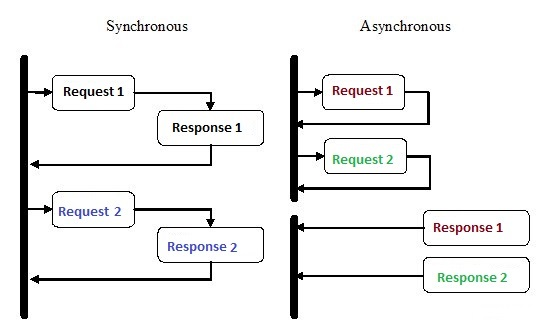
\includegraphics[width=1.0\columnwidth]{sync} 
	\caption{Illustazione della differenza tra chiamate sincrone ed asincrone}
\end{figure}
\newpage
\section{Aspettative Aziendali}
Al termine delle 340 ore l'azienda si aspetta di avere un libreria di filtraggio solida ed estendibile, in grado di eseguire le principali funzionalità di filtraggio al'interno di un log degli eventi e un'interfaccia \textit{frontend} semplice ed intuitiva in grado di utilizzare tutte le funzionalità incluse all'interno della libreria.
Il tutto deve essere pensato per un’erogazione in modalità \textit{cloud}, pertanto le scelte architetturali dovranno tener conto di questo prerequisito.
\begin{figure}[!h] 
	\centering 
	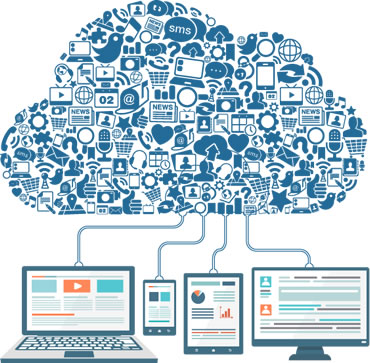
\includegraphics[width=0.3\columnwidth]{cloud} 
	\caption{Illustazione semplificata di un'architettura server cloud}
\end{figure}
Tali attività mi hanno portato a definire i principali requisiti con il tutor aziendale, che sono poi stati inseriti all'interno del piano di lavoro. In seguito a ciò il tutor ha individuato gli obiettivi per il progetto suddividendoli in due categorie: obbligatori e desiderabili.\\
\\
\\
\begin{table}[!h]
	\caption{Obiettivi obbligatori dello Stage}
\begin{tabularx}{\textwidth}{lXl}
	\hline\hline
	\textbf{Obiettivi obbligatori}\\
	\hline
	Inquadramento del problema: stesura di un documento di specifica del problema\\
	affrontato; &  \\
	\hline
	\hline
     Analisi dei requisiti e specifiche tecniche di progettazione: stesura dei relativi\\
     documenti; &  \\
	\hline
	\hline
	Implementazione del frontend web e dei servizi di backend necessari a gestire le\\
	funzionalità di filtraggio degli eventi &  \\
	\hline
	\hline
	Collaudo del sistema: il progetto deve prevedere una fase di test del software\\
	implementato, con documentazione dei risultati ottenuti &  \\
	\hline	
\end{tabularx}
\end{table}
\begin{table}[!h]
	\caption{Obiettivi desiderabili dello Stage}
	\begin{tabularx}{\textwidth}{lXl}
		\hline\hline
		\textbf{Obiettivi desiderabili}\\
		\hline
		point-and-click sul processo per inserimento di filtri sulle successioni di eventi&  \\
		\hline
		\hline
		implementazione test frontend &  \\
		\hline
	\end{tabularx}
\end{table}
\subsection{Vincoli}
I vincoli che mi sono stati posti durante la stesura del piano di lavoro possono essere raggruppati in 3 categorie:
\subsubsection{Vincoli temporali}
Rappresentano i vincoli dal punto di vista del tempo. Lo svolgimento dello stage ha avuto una durata di 340 ore. Tali ore sono state dstribuite in modo uniforme durante l'arco di 9 settimane. Inizialmente sono state concordate 8 settimane, ma in seguito ad alcune criticità riscontrate in fase di sviluppo, con la conseguente negoziazione dei requisiti, sono state portate a 9; includendo quindi una settimana aggiuntiva per terminare tutte le attività concordate.
Nel periodo antecedente all'inizio dello stage l'azienda ha redatto una scansione temporale delle attività su base settimanale suddivisa nel seguente modo:
\begin{itemize}
	\item \textbf{Settimana 1}: Studio introduttivo del Process Mining con le relative tecnologie. Studio dell’architettura di storage messa a disposizione e del	framework ProM
	\item \textbf{Settimana 2}: Studio di fattibilità per la realizzazione dei moduli necessari a erogare le funzionalità di filtraggio
    \item \textbf{Settimana 3-4-5}: Progettazione dei moduli di discovery del processo, visualizzazione log e filtraggio
    \item \textbf{Settimana 6-7}: Implementazione del software e deploy su docker
    \item \textbf{Settimana 8}: Test e sperimentazione del software
\end{itemize}
Durante tutto l'arco delle settimane è stata richiesta anche una documentazione sul lavoro includendo una breve cronologia delle attività svolte, indicando le eventuali criticità riscontrate e specificando in che modo sono state affrontate e risolte.\\
Tale pianificazione è stata rinegoziata a partire dalla sesta settimana; in quanto l'architettura finale non era stata ancora ideata in modo specifico. Questo ha portato, in accordo con il tutor ad una rinegoziazione dei requisiti e quindi della attività programmate; sostituendo il \textit{deploy} su \textit{docker} con l'implmentazione di alcuni stub in modo da poter effettuare test lato frontend.
\begin{figure}[!h] 
	\centering 
	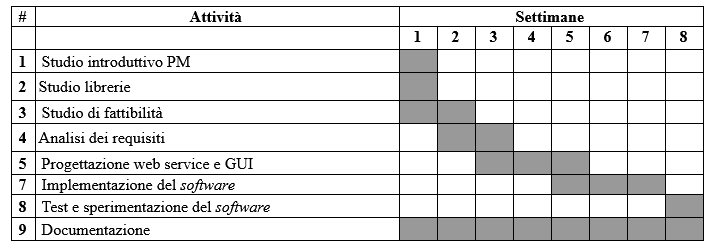
\includegraphics[width=1.0\columnwidth]{gantt} 
	\caption{Diagramma di gantt relativo alle attività di stage}
\end{figure}
\subsubsection{Vincoli metodologici}
Lo stage è stato svolto presso la sede di Rubano(PD) in comune accordo con il tutor. Ciò è stato deciso con lo scopo di poter confrantarsi ed interagire in maniera sistematica ogni qualvolta ce ne fosse stato bisogno; non soltanto tramite un rapporto stagista e tutor, ma confrontandosi con altri figure presenti all'interno dell'azienda in modo da poter consolidare nuovi rapporti di tipo professionale, in modo da avere supporto aggiuntivo in caso ce ne fosse stata necessità.
Oltre a ciò è stato richiesto un continuo confronto sulle attività effettuate e quelle in programma tramite alcune note di testo condivise tra il tutor ed il team di Ricerca e Sviluppo.
Tali note sono poi oggetto di discussione tramite \textit{Daily meeting}: in cui vi è un momento di confronto tra i membri dei team per discutere in merito alle attività svolte e quelle in programma per la giornata. Mi stata messa a disposizione una postazione di lavoro con personal computer, connessione ad Internet ed alla rete locale con accesso al server di sviluppo, in modo da poter effettuare \textit{\gls{deploy}} di eventuali macchine virtuali necessarie allo sviluppo. Sono stati forniti una serie dati di esempio per testare quanto sviluppato, oltre a tutte le librerie necessarie allo sviluppo stesso dell’applicativo.
\begin{figure}[!h] 
	\centering 
	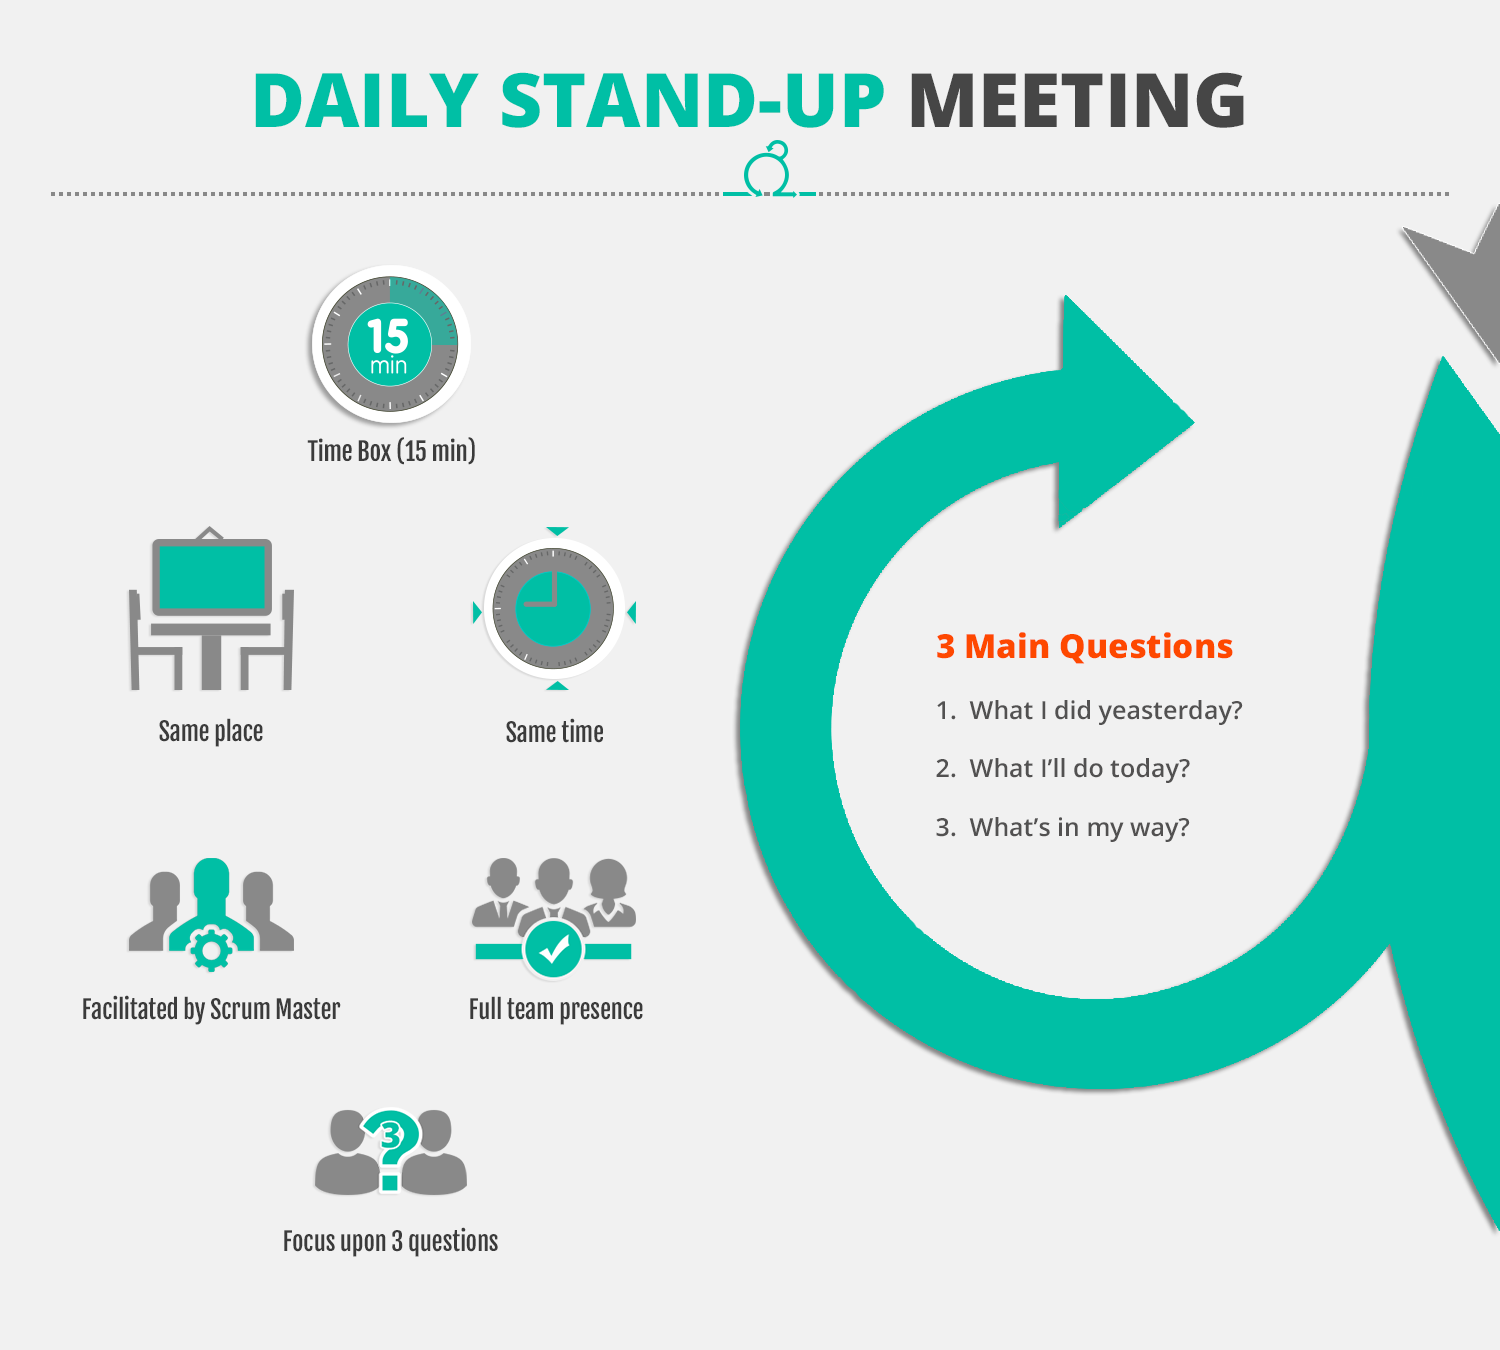
\includegraphics[width=0.95\columnwidth]{daily} 
	\caption{Illustrazione semplificata di \textit{Daily Meeting}}
\end{figure}
\subsubsection{Vincoli tecnologici}
Come sopra descritto l'obiettivo fondamentamentale per l'azienda è che l'applicativo finale fosse in grado di girare su server \textit{Cloud}. Questo ha influito in modo significativo sui vincoli tecnologici che sono stati imposti. Innanzitutto tramite lo sviluppo di una libreria che fosse scritta in modo semplice e leggibile, per far sì che chi dovrà inserirla nell'ambiente a microservizi abbia un'idea precisa delle sue caratterische ed il suo funzionamento; in secondo luogo tramite la gestione dell'asincronia all'interno dell'interfaccia \textit{frontend}, andando a gestire i messaggi in arrivo del server, categorizzandoli e cambiando il comportamente dell'interfaccia a seconda della caratterizzazione del messaggio.
\section{Aspettative Personali}
Tutte le mie passate esperienze sono riconducibili esclusivamento all'ambito accademico; l'esperienza che più mi ha avvicinato all'ambito lavorativo è stato il progetto di Ingegneria del Software; tramite il quale ho potuto constatare alcune dinamiche presenti all'interno di un contesto professionale. Per poter approcciarmi al mondo lavorativo ho partecipato all'evento organizzato dall'Università di Padova \textit{Stage-IT} tramite il quale ho potuto affrontare diversi incontri con realtà aziendali ben formate e strutturate. Durante la fiera ho potuto valutare diverse attività di stage tenendo in considerazione le tematiche trattate e quanto ciò potessero incidere nel mio grado di formazione. La maggior parte di esse non sono risultate, a mio parere, stimolanti per la mia maturità a livello professionale. 
Le aspettative che mi sono preposto prima dell'evento di \textit{Stage-IT} sono state le seguenti:
\begin{itemize}
	\item Apprendimento di nuove metodologie di lavoro
	\item Visione e apprendimento di nuove tecnologie
	\item Lavoro in modo autonomo sotto la supervisione che tutor che mi presti supporto
	\item Visione del contesto lavorativo in maniera più ampia, non legata strettamente all'attività di stage
\end{itemize}
Successivamente a \textit{Stage-IT} sono stato contattato da altre aziende operanti nel settore dell'informatica, ognuna delle quali mi ha proposto varie attività affrontando diversi argomenti e tecnologie.
Una su tutte che mi ha colpito è stata proprio \textit{Siav} che, attraverso le loro proposte e la loro costante dedizione in merito alla ricerca di nuove tematiche e tecnologie mi ha convinto a svolgere l'attività di stage presso la loro azienda, collocandomi proprio all'interno del team di Ricerca e Sviluppo. Ciò ha comportato un aumento delle mie aspettative di fronte a questa attivita:
\begin{itemize}
	\item Valutare quanto possano essermi state utili le nozioni apprese durante il percorso universitario.
	\item apprendimento di nuove tecnologie
	\item Apprendimento dei principi cardine del process mining
	\item Apprendimento sul funzionamento di un'architettura a microservizi 
	\item Instaurazione di discussioni con il personale in modo da potersi confrontare ed avere diversi punti di vista rispetto ad alcune tematiche
	
\end{itemize}
             % Processi
% !TEX encoding = UTF-8
% !TEX TS-program = pdflatex
% !TEX root = ../tesi.tex

%**************************************************************
\chapter{Resoconto dello stage}
\label{cap:descrizione-stage}
%**************************************************************

\intro{In questo capitolo andrò a descrivere i principali aspetti che sono stati affrontati durante lo stage}\\

%**************************************************************
\section{Introduzione al progetto}
Visto in scala più ampia, il progetto finale risulterà una rivisitazione di Bipod, un applicativo di Siav, in ambito process mining, utilizzato come gestore di processi aziendali.
Tale software, dopo averlo provato con mano, risulta funzionale in ogni sua parte, anche se la sua struttura risulta poco estendibile. Per questo motivo mi è stato proposto di sviluppare una parte di software che si andrà poi ad integrare con il nuovo applicativo che adrà a rimpiazzare l'attuale esistente.
Nello specifico le richieste a cui ho fatto fronte sono state le seguenti:
\begin{itemize}
	\item Libreria di process mining per filtraggio su log degli eventi.
	\item Interfaccia fronted tenendo come punto di riferimento il vecchio applicativo.
	\item Stub per verificare il correntto comportamento dell'interfaccia di filtraggio
\end{itemize}
\section{Pianificazione del progetto}
Durante il periodo antecedente all'inizio dell'attività di progetto sono state discusse con il tutor tutte le principali che attività che avrei dovuto svolgere nell'arco dei due mesi preposti. Tali attività, anche se in forma generica, sono state inserite nel diagramma di Gantt presente al capitolo precedente (Figura 2.3).
Per tener traccia di tutte le attività svolte duraurante il periodo di stage, tramite il supporto del tutor e del team in cui sono stato inserito ho cercato di apprendere nella miglior maniera possibile i principi cardine dell'\textit{Agile programming}. Non avendo mai avuto l'occasione prima d'ora di approcciarmi a tale metodologia è stato impegnativo, ma appagante entrare nei suoi meccanismi pratici e nelle sue dinamiche. Tuttavia sono riuscito, almeno in parte, a comprendere alcune importanti metodologie che sono state applicate durante tutto il periodo di stage. Le attività sono state tracciate tramite semplici note, condivise con l'interno team, in cui è descritta un breve cronologia di tutte le attività svolte giorno per giorno, indicando eventuali problematiche riscontrate e come sono state affrontate.

\section{Analisi dei requisiti}

\section{Progettazione}
\subsection{Libreria}
\subsection{Frontend}
\section{Codifica}
\section{Verifica}
\section{Validazione}
\section{Copertura}
             % Kick-Off
% !TEX encoding = UTF-8
% !TEX TS-program = pdflatex
% !TEX root = ../tesi.tex

%**************************************************************
\chapter{Analisi dei requisiti}
\label{cap:analisi-requisiti}
%**************************************************************

\intro{Breve introduzione al capitolo}\\

\section{Casi d'uso}

Per lo studio dei casi di utilizzo del prodotto sono stati creati dei diagrammi.
I diagrammi dei casi d'uso (in inglese \emph{Use Case Diagram}) sono diagrammi di tipo \gls{uml} dedicati alla descrizione delle funzioni o servizi offerti da un sistema, così come sono percepiti e utilizzati dagli attori che interagiscono col sistema stesso.
Essendo il progetto finalizzato alla creazione di un tool per l'automazione di un processo, le interazioni da parte dell'utilizzatore devono essere ovviamente ridotte allo stretto necessario. Per questo motivo i diagrammi d'uso risultano semplici e in numero ridotto.

\begin{figure}[!h] 
    \centering 
    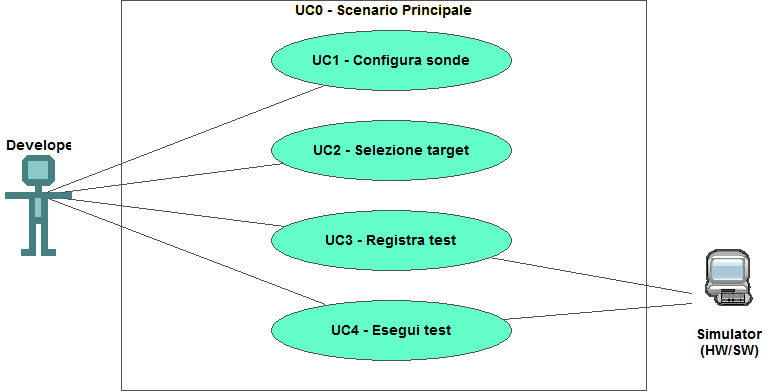
\includegraphics[width=0.9\columnwidth]{usecase/scenario-principale} 
    \caption{Use Case - UC0: Scenario principale}
\end{figure}

\begin{usecase}{0}{Scenario principale}
\usecaseactors{Sviluppatore applicativi}
\usecasepre{Lo sviluppatore è entrato nel plug-in di simulazione all'interno dell'IDE}
\usecasedesc{La finestra di simulazione mette a disposizione i comandi per configurare, registrare o eseguire un test}
\usecasepost{Il sistema è pronto per permettere una nuova interazione}
\label{uc:scenario-principale}
\end{usecase}

\section{Tracciamento dei requisiti}

Da un'attenta analisi dei requisiti e degli use case effettuata sul progetto è stata stilata la tabella che traccia i requisiti in rapporto agli use case.\\
Sono stati individuati diversi tipi di requisiti e si è quindi fatto utilizzo di un codice identificativo per distinguerli.\\
Il codice dei requisiti è così strutturato R(F/Q/V)(N/D/O) dove:
\begin{enumerate}
	\item[R =] requisito
    \item[F =] funzionale
    \item[Q =] qualitativo
    \item[V =] di vincolo
    \item[N =] obbligatorio (necessario)
    \item[D =] desiderabile
    \item[Z =] opzionale
\end{enumerate}
Nelle tabelle \ref{tab:requisiti-funzionali}, \ref{tab:requisiti-qualitativi} e \ref{tab:requisiti-vincolo} sono riassunti i requisiti e il loro tracciamento con gli use case delineati in fase di analisi.

\newpage

\begin{table}%
\caption{Tabella del tracciamento dei requisti funzionali}
\label{tab:requisiti-funzionali}
\begin{tabularx}{\textwidth}{lXl}
\hline\hline
\textbf{Requisito} & \textbf{Descrizione} & \textbf{Use Case}\\
\hline
RFN-1     & L'interfaccia permette di configurare il tipo di sonde del test & UC1 \\
\hline
\end{tabularx}
\end{table}%

\begin{table}%
\caption{Tabella del tracciamento dei requisiti qualitativi}
\label{tab:requisiti-qualitativi}
\begin{tabularx}{\textwidth}{lXl}
\hline\hline
\textbf{Requisito} & \textbf{Descrizione} & \textbf{Use Case}\\
\hline
RQD-1    & Le prestazioni del simulatore hardware deve garantire la giusta esecuzione dei test e non la generazione di falsi negativi & - \\
\hline
\end{tabularx}
\end{table}%

\begin{table}%
\caption{Tabella del tracciamento dei requisiti di vincolo}
\label{tab:requisiti-vincolo}
\begin{tabularx}{\textwidth}{lXl}
\hline\hline
\textbf{Requisito} & \textbf{Descrizione} & \textbf{Use Case}\\
\hline
RVO-1    & La libreria per l'esecuzione dei test automatici deve essere riutilizzabile & - \\
\hline
\end{tabularx}
\end{table}%             % Concept Preview
%% !TEX encoding = UTF-8
% !TEX TS-program = pdflatex
% !TEX root = ../tesi.tex

%**************************************************************
\chapter{Progettazione e codifica}
\label{cap:progettazione-codifica}
%**************************************************************

\intro{Breve introduzione al capitolo}\\

%**************************************************************
\section{Tecnologie e strumenti}
\label{sec:tecnologie-strumenti}

Di seguito viene data una panoramica delle tecnologie e strumenti utilizzati.

\subsection*{Tecnologia 1}
Descrizione Tecnologia 1.

\subsection*{Tecnologia 2}
Descrizione Tecnologia 2

%**************************************************************
\section{Ciclo di vita del software}
\label{sec:ciclo-vita-software}

%**************************************************************
\section{Progettazione}
\label{sec:progettazione}

\subsubsection{Namespace 1} %**************************
Descrizione namespace 1.

\begin{namespacedesc}
    \classdesc{Classe 1}{Descrizione classe 1}
    \classdesc{Classe 2}{Descrizione classe 2}
\end{namespacedesc}


%**************************************************************
\section{Design Pattern utilizzati}

%**************************************************************
\section{Codifica}
             % Product Prototype
%% !TEX encoding = UTF-8
% !TEX TS-program = pdflatex
% !TEX root = ../tesi.tex

%**************************************************************
\chapter{Verifica e validazione}
\label{cap:verifica-validazione}
%**************************************************************             % Product Design Freeze e SOP
%% !TEX encoding = UTF-8
% !TEX TS-program = pdflatex
% !TEX root = ../tesi.tex

%**************************************************************
\chapter{Conclusioni}
\label{cap:conclusioni}
%**************************************************************

%**************************************************************
\section{Consuntivo finale}

%**************************************************************
\section{Raggiungimento degli obiettivi}

%**************************************************************
\section{Conoscenze acquisite}

%**************************************************************
\section{Valutazione personale}
             % Conclusioni
\appendix                               
%% !TEX encoding = UTF-8
% !TEX TS-program = pdflatex
% !TEX root = ../tesi.tex

%**************************************************************
\chapter{Appendice A}
%**************************************************************

\epigraph{Citazione}{Autore della citazione}



             % Appendice A

%**************************************************************
% Materiale finale
%**************************************************************
\backmatter
\printglossaries
% !TEX encoding = UTF-8
% !TEX TS-program = pdflatex
% !TEX root = ../tesi.tex

%**************************************************************
% Bibliografia
%**************************************************************

\cleardoublepage
\chapter{Bibliografia}
\textbf{\Large Siti web consultati}\\\\
\textit{Metodologia Agile}: \url{https://it.wikipedia.org/wiki/Metodologia_agile}\\\\
\textit{Angular}: \url{https://angular.io/}\\\\
\textit{Framework Angular material:} \url{https://material.angular.io}\\\\
\textit{Bipod:} \url{ https://www.siav.com/it/soluzioni-software/bipod-applicativo-process-mining/}\\\\
\textit{Disco software}: \url{https://fluxicon.com/disco/}\\\\
\textit{Docker}: \url{https://www.docker.com}\\\\
\textit{Javadoc}: \url{ https://docs.oracle.com/javase/8/docs/technotes/tools/windows/javadoc.html}\\\\
\textit{Standard OpenXES}: \url{http://www.xes-standard.org/openxes/start}\\\\
\textit{ProM}: \url{www.promtools.org}\\\\
\textit{RabbitMQ}: \url{https://www.rabbitmq.com/}\\\\
	\textit{Libreria RxJS}: \url{https://rxjs-dev.firebaseapp.com/}\\\\
	\textit{Siav Spa}: \url{https://www.siav.com}\\\\
	\textit{Stage-IT}: \url{http://informatica.math.unipd.it/laurea/stageit.html}\\\\
	\textit{Team Foundation Server}: \url{https://en.wikipedia.org/wiki/Azure_DevOps_Server}\\\\
	\textit{Team Foundation Version Control}: \url{https://docs.microsoft.com/it-it/visualstudio/mac/tf-version-control?view=vsmac-2019}\\\\
\nocite{*}



\end{document}
